\documentclass[12pt,a4paper]{article}
\usepackage[utf8]{inputenc}
\usepackage[T1]{fontenc}
\usepackage[english]{babel}
\usepackage{graphicx}
\usepackage{hyperref}
\usepackage[x11names]{xcolor}
\usepackage{fancyhdr}
\usepackage[margin=2cm]{geometry}
\usepackage{minted}
\graphicspath{{./imatges/}}% Lloc on hi ha els logos


\lhead{ESII Pràctica 1, curs 2023/24 GDDV-GEINF}
\rhead{\thepage}
\cfoot{}
\begin{document}
    \begin{titlepage}
        \newcommand{\HRule}{\rule{\linewidth}{0.5mm}} % Defines a new command for the horizontal lines, change thickness here
        \begin{flushleft}
            
\includegraphics[height=1.5cm]{EPS.png}\\\vfill
        \end{flushleft}
        \center % Center everything on the page
        %----------------------------------------------------------------------------------------
        %	HEADING SECTIONS
        %----------------------------------------------------------------------------------------
        \textsc{\huge \bfseries Pràctiques ESII}\\[0.25cm]
        \textsc{\Large \bfseries Curs 2023/24}\\[0.25cm]
        \textsc{\large GEINF- GDDV }
        %----------------------------------------------------------------------------------------
        %	TITLE SECTION
        %----------------------------------------------------------------------------------------
        \HRule \\[0.4cm]
        { \huge \bfseries Pràctica 1} \\[0.4cm] % Title of your document
Grup T \\ Jordi Badia, Aniol Juanola i Guillem Vidal
        \HRule \\\vfill
        \begin{minipage}{0.4\textwidth}
            \begin{flushleft}
                
\includegraphics[height=1.5cm]{KairoMart}
            \end{flushleft}
        \end{minipage}
        \hfill
        \begin{minipage}{0.4\textwidth}
            \begin{flushright} \large
                {\small (\today)}
            \end{flushright}
        \end{minipage}
    \end{titlepage}


\tableofcontents

\clearpage


\section{Use case diagram}

\begin{figure}[ht]
    \centering
    \includegraphics[width=\textwidth]{Diagrama de casos d'ús.png}
\end{figure}

\newpage

\subsection{Use case sheet ``Drive in a race''}

\begin{figure}[ht]
    \centering
    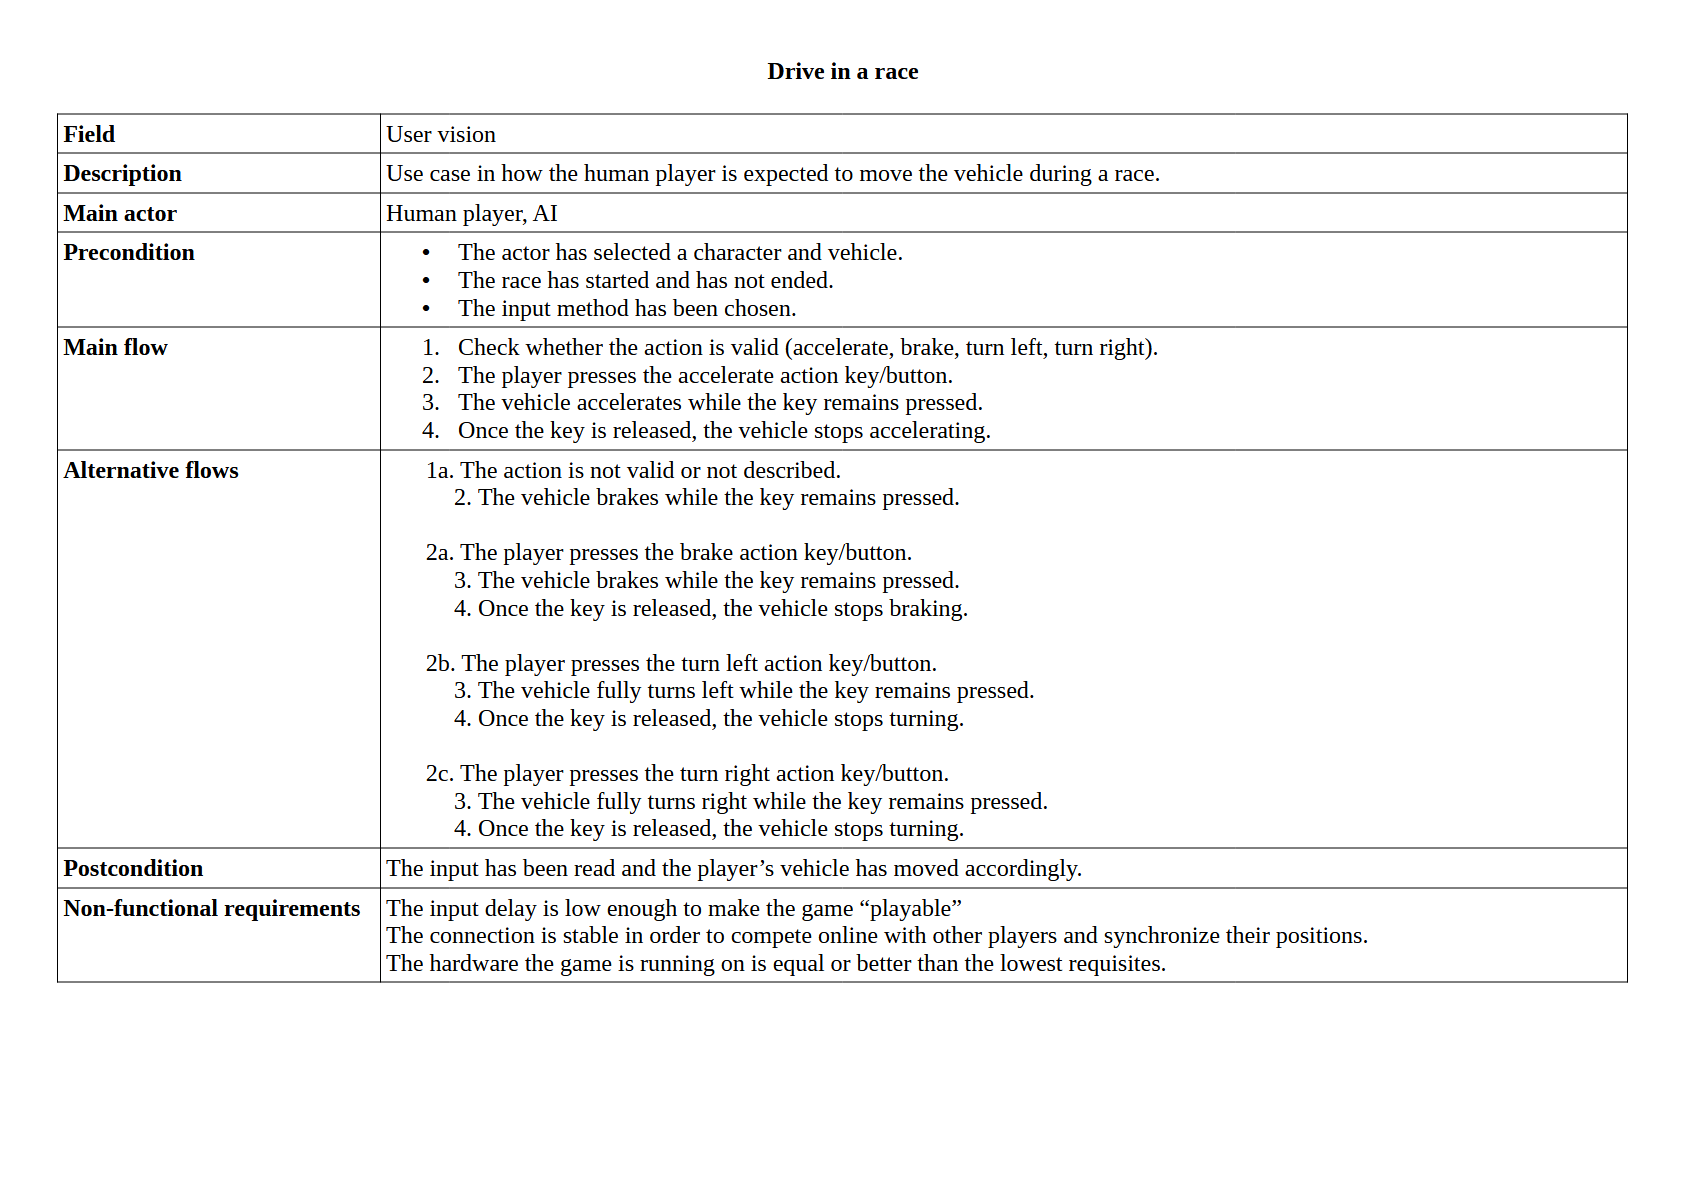
\includegraphics[width=\textwidth]{Fer moure vehicle - Use case.png}
\end{figure}

\subsection{Use case sheet ``Show classification''}

\begin{figure}[ht]
    \centering
    \includegraphics[width=\textwidth]{Mostrar classificació - Use case.png}
\end{figure}

\newpage

\section{Class diagram}

\begin{figure}[ht]
    \centering
    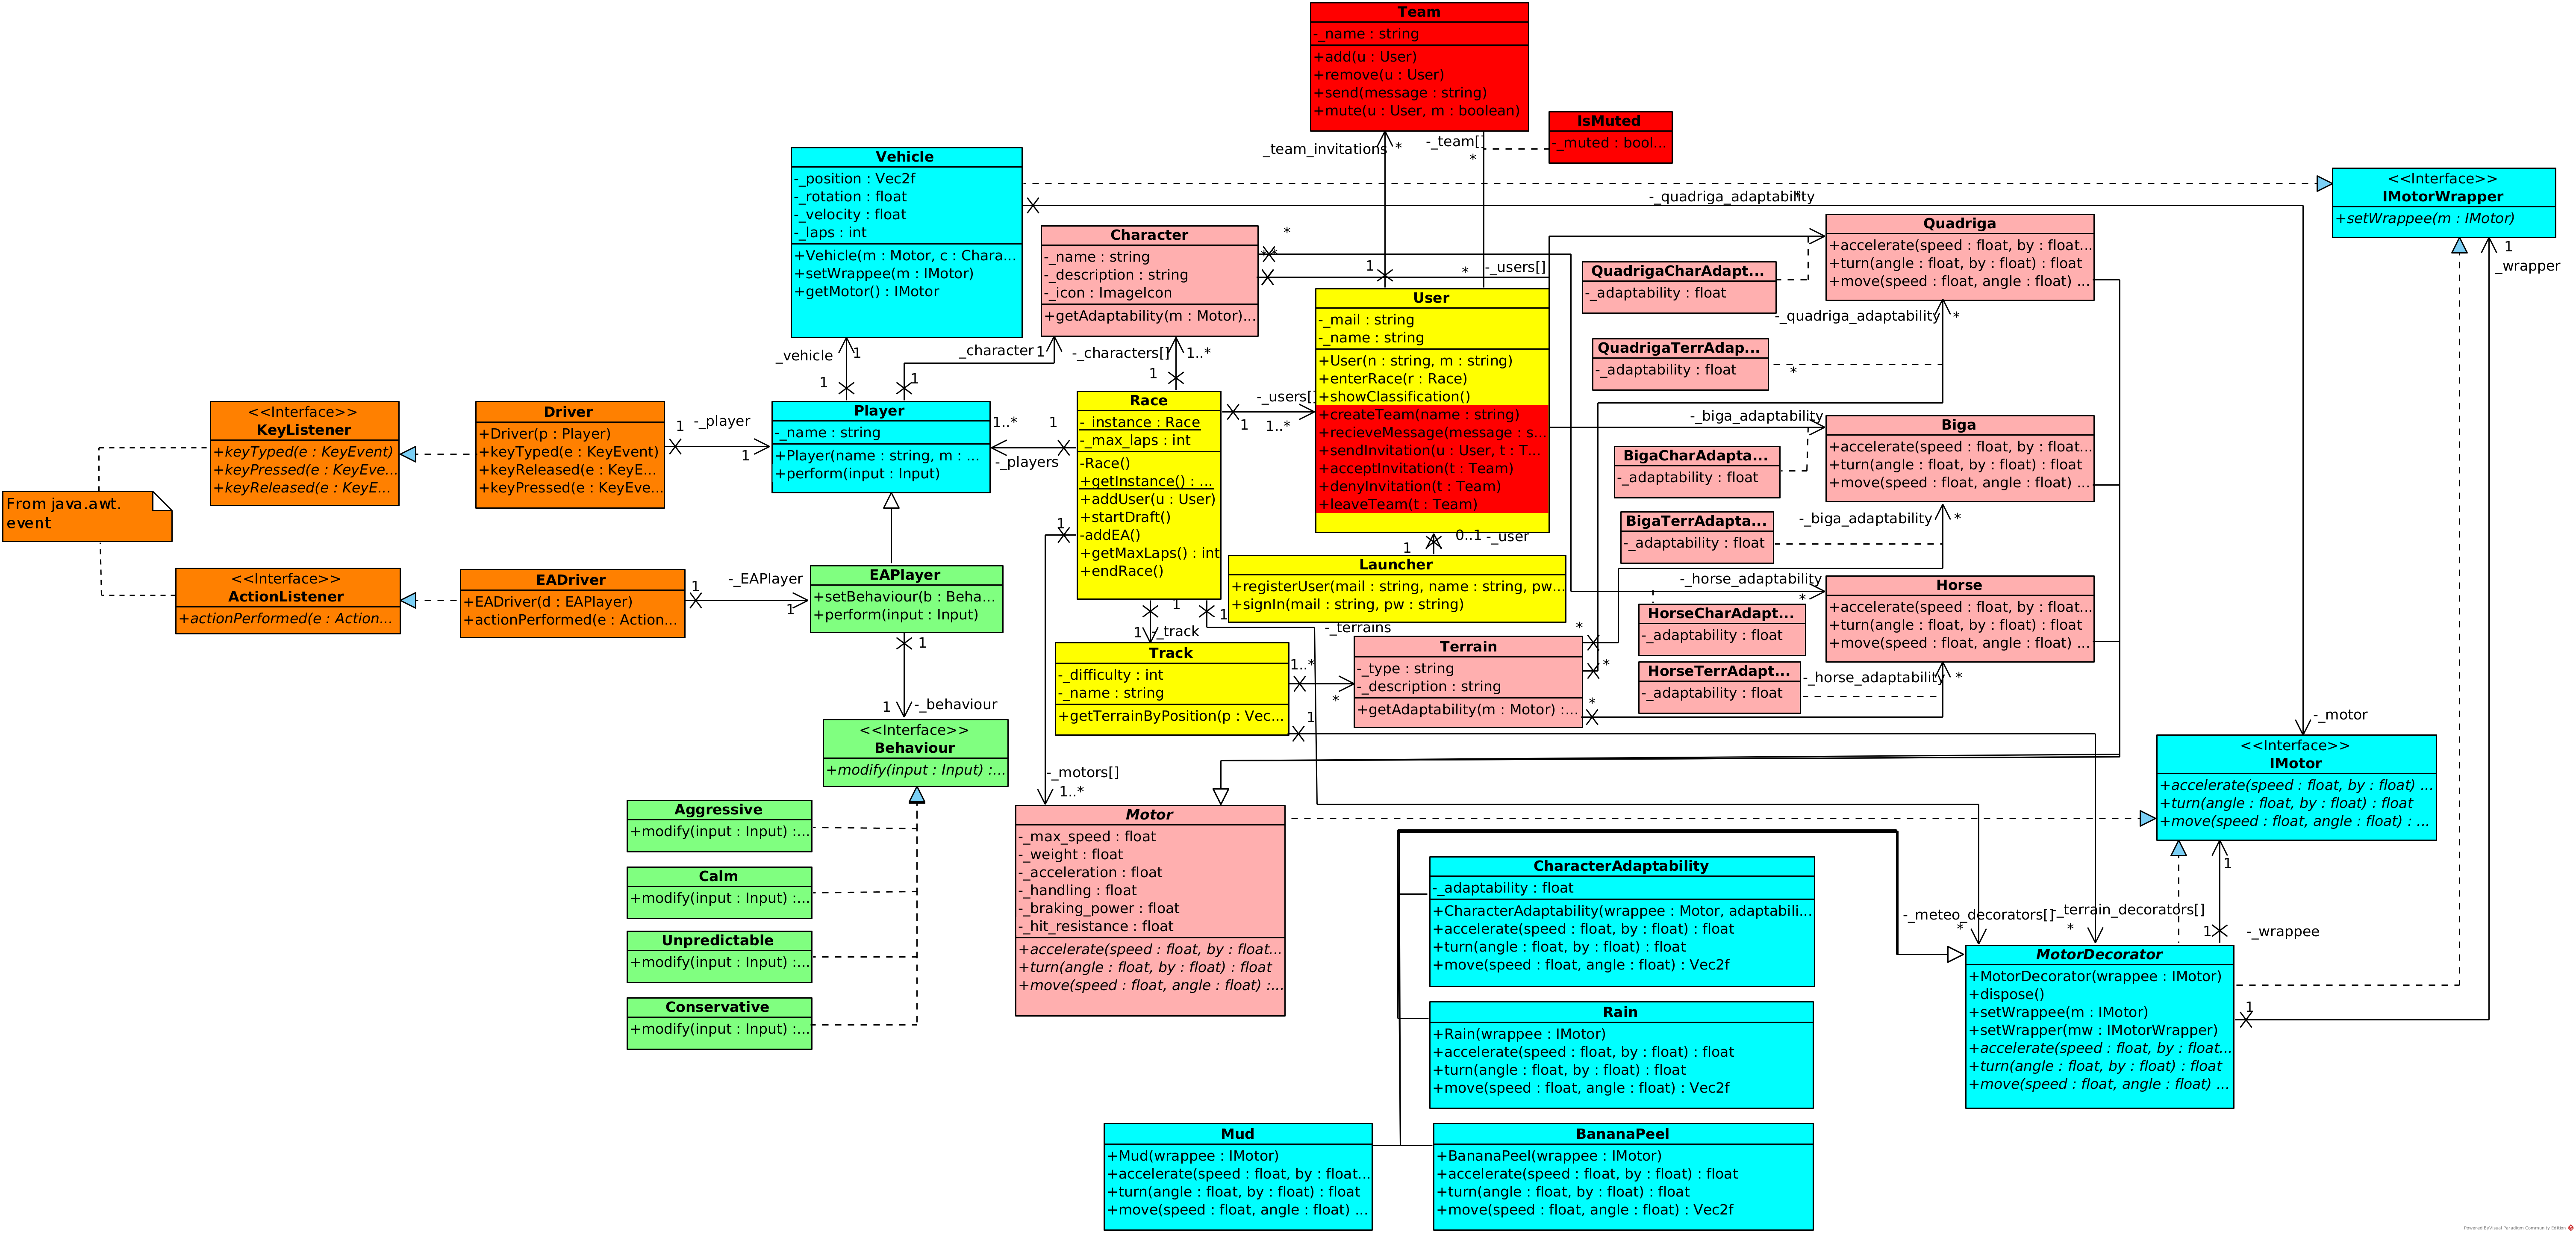
\includegraphics[width=\textwidth]{Diagrama de Classes.png}
\end{figure}

\begin{description}
    \item[Green] strategy pattern to determine EA's behaviour. The function \mintinline{Java}{Modify(Input)} alters the EA's intention and \mintinline{Java}{setBehaviour(Behaviour)} changes the behaviour itself.
    \item[Orange] interfaces and their implementations regarding player input.
    \item[Yellow] miscellaneous classes.
    \begin{itemize}
        \item Race can be understood as the lobby of the execution. One can add users to the race, and the remaining space will be filled by EAs. Then, all players must choose both the character and the vehicle they are going to play with. And with that the race can begin. Race manages the instances of motor and character, which are unchanging and shared between players. When a vehicle has completed a \mintinline{Java}{_max_laps} number of laps, the race ends.
        \item User contains the information of the client (name, email...).
        \item Launcher is the client: log ins and sign ups go through this class. The password is not stored in the User class, instead Launcher uses it to identify the user in the database.
    \end{itemize}
    \item[Pink] constant classes of characters, motors, terrains and adaptabilities.\footnote{Adaptability classes will be implemented as maps.}
    \item[Blue] all the classes that store the current state of the race in relation to each player (position, rotation, velocity). Effects are applied on vehicles via decorators, either character or terrain adaptabilities, atmospheric conditions or in-game items (such as banana peels or mushrooms). In order to erase an effect, decorators, being linked lists, must be doubly linked. The \mintinline{Java}{IMotorWrapper} interface allows decorators to be treated as nodes in a list, and vehicle, being an end point of the list, implements it as well.
\end{description}

\newpage

\section{EER diagram}

\begin{figure}[ht]
    \centering
    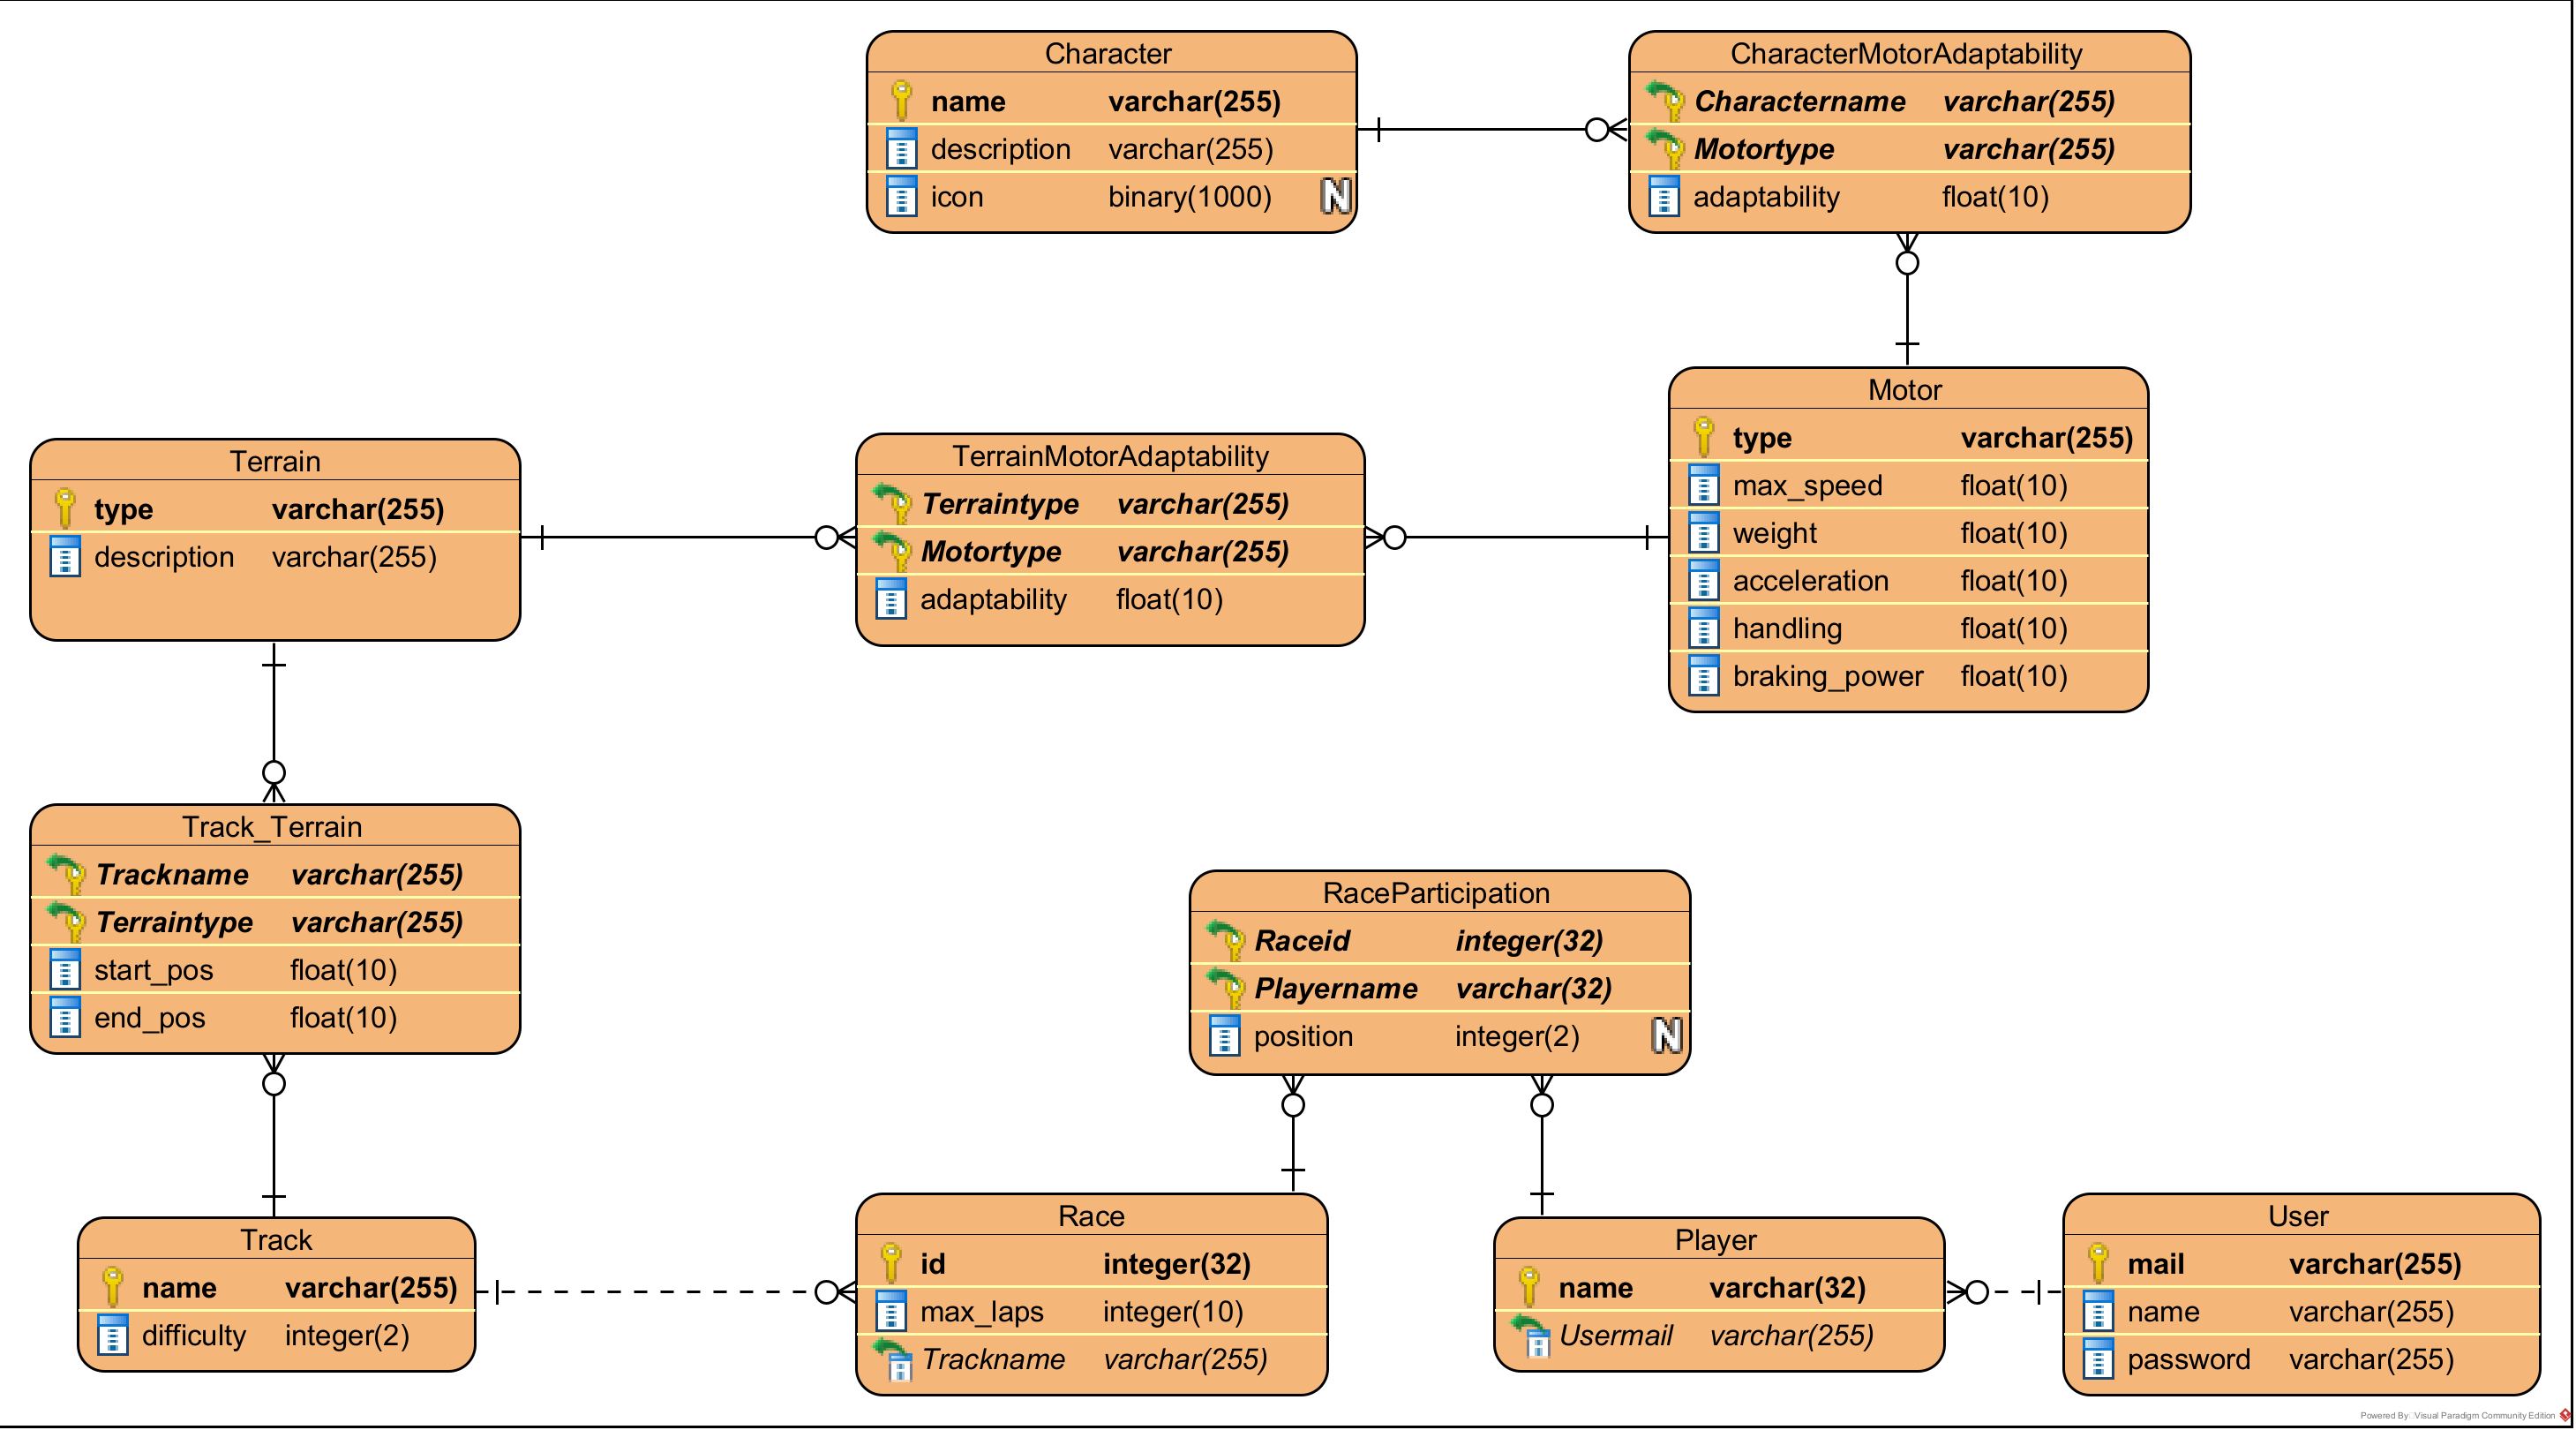
\includegraphics[width=\textwidth]{Entity Relationship Diagram.png}
\end{figure}

This diagram represents what one would store in a real database, i.e. there's no information about the current state of the game but its persistent data.

\end{document}